% \documentclass{article}
% \usepackage[english]{babel}
% \usepackage{amsmath,amssymb,graphicx,alltt}

%%%%%%%%%% Start TeXmacs macros
\newcommand{\tmop}[1]{\ensuremath{\operatorname{#1}}}
\newcommand{\tmtextbf}[1]{\text{{\bfseries{#1}}}}
\newenvironment{tmindent}{\begin{tmparmod}{1.5em}{0pt}{0pt}}{\end{tmparmod}}
\newenvironment{tmparmod}[3]{\begin{list}{}{\setlength{\topsep}{0pt}\setlength{\leftmargin}{#1}\setlength{\rightmargin}{#2}\setlength{\parindent}{#3}\setlength{\listparindent}{\parindent}\setlength{\itemindent}{\parindent}\setlength{\parsep}{\parskip}} \item[]}{\end{list}}
%%%%%%%%%% End TeXmacs macros
\section{Notes}
\subsection{Twelvethfold Way}

\raisebox{0.0\height}{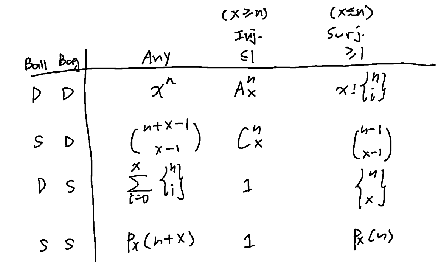
\includegraphics[width=7.4370818575364cm,height=4.49781910009183cm]{/home/xade/icpc/kactl/content/combinatorial/comb_notes-1.pdf}}

\subsection{Identities on C}

\tmtextbf{Vandermonde's Id. }$\binom{m + n}{k} = \sum_{r \in [0, k]}
\binom{m}{r} \binom{n}{k - r}$

\tmtextbf{Pascal's Rule. }$\binom{n}{k} = \binom{n - 1}{k - 1} + \binom{n -
1}{k}$

\tmtextbf{Hockey Stick Id. }sum n over same k
\begin{tmindent}
  $\sum_{i \in [r, n]} \binom{i}{r} = \binom{n + 1}{r + 1}  \forall n, r \in
  \mathbb{N}, n \geqslant r$
\end{tmindent}
\tmtextbf{Binomial Theorem. }$(x + y)^n = \sum_{k \in [0, n]} C_n^k \cdot x^{n
- k} \cdot y^k$

\tmtextbf{Stirling's Approximation. }$n! \approx \sqrt{2 \pi n} \left(
\frac{n}{e} \right)^n$ with error $\frac{1}{n + 1}$

\tmtextbf{Lucas Theorem. }$\binom{n}{k} \tmop{mod} p = \prod \binom{n_i}{k_i}
\tmop{mod} p$
\begin{tmindent}
  Convention is $C (n, k) = 0$ if $k > n$.
  Corollary. mod = 0 iff there is a digit of n greater than k.
\end{tmindent}

\subsection{Other Basic Comb Functions}

\tmtextbf{Stirling number of first kind. }Count number of permutations on n
item with k cycles.
\begin{tmindent}
  $c (n, k) = c (n - 1, k - 1) + (n - 1) c (n - 1, k)$
  
  $c (0, 0) = 1$
  
  $\sum_{k = 0}^n c (n, k) x^k = x (x + 1) \ldots (x + n - 1)$
  
  c(8,k)=8,0,5040,13068, c(n,2)=0,0,1,3,11
\end{tmindent}
\tmtextbf{Eulerian Numbers. }Number of permutation s.t. exactly k elems are
greater than prev elem.
\begin{tmindent}
  $E (n, k) = (n - k) E (n - 1, k - 1) + (k + 1) E (n - 1, k)$
  
  $E (n, 0) = E (n, n - 1) = 1$
  
  $E (n, k) = \sum_{j = 0}^k (- 1)^j \binom{n + 1}{j} (k + 1 - j)^n$
\end{tmindent}
\tmtextbf{Stirling Number of second kind. }Partition of n distinct numbers
into exact k group.
\begin{tmindent}
  $S (n, k) = S (n - 1, k - 1) + \tmop{kS} (n - 1, k)$
  
  $S (n, 1) = S (n, n) = 1$
  
  $S (n, k) = \frac{1}{k!} \sum_{i \in [0, k]} (- 1)^{k - i} \binom{k}{i} i^n
  = \sum_{i = 0}^k \frac{(- 1)^{k - i} i^n}{i! (k - i) !}$
  \begin{verbatim}
    ll S2(ll n, ll k) \{
      ll ans = 0;
      FOR(i, 0, k) \{
       ll sgn = ((k - i) % 2 ? -1 : 1);
       ll in = fpm(i, n, p);
       ll bottom = invfac[i] * invfac[k - i] % p;
       ans = (ans + sgn * in * bottom % p) % p;
      \}
      return (ans % p + p) % p;
    \}
  \end{verbatim}
  
\end{tmindent}
\tmtextbf{Bell number. }Number of partition of n distinct nums.
\begin{tmindent}
  $B (n) = 1, 1, 2, 5, 15, 52 \ldots$
  
  For prime $p$, $B (p^m + n) \equiv \tmop{mB} (n) + B (n + 1) \quad
  \tmop{mod} \quad p$
\end{tmindent}
\tmtextbf{Partition Function. }Number of ways of writing $n$ as sum of
positive integers, disregarding order of summands.
\begin{tmindent}
  $p (0) = 1, p (n) = \sum_{k \in [- \inf, 0) \cup (0, \inf]} (- 1)^{k + 1} p
  (n - k (3 k - 1) / 2)$
  
  $p (n) \sim 0.145 / n \cdot \exp \left( 2.56 \sqrt{n} \right)$
  
  $p = 1, 1, 2, 3, 5, 7, 11, 15, 22, 30, p (20) = 627, p (50) \approx 2 e 5, p
  (100) \approx 2 e 8$
\end{tmindent}

\subsection{Misc Functions}

\tmtextbf{Derangements. }$D (n) = (n - 1) (D (n - 1) + D (n - 2)) = \tmop{nD}
(n - 1) + (- 1)^n = \lfloor \frac{n!}{e} \rceil$

\tmtextbf{Catalan Numbers. }Various
\begin{tmindent}
  $C_n = \frac{1}{n + 1} \binom{2 n}{n} = \binom{2 n}{n} - \binom{2 n}{n + 1}
  = \frac{(2 n) !}{(n + 1) !n!}$
  
  $C_0 = 1, C_{n + 1} = \frac{2 (2 n + 1)}{n + 2} C_n, C_{n + 1} = \sum C_i
  C_{n - i}$
  
  $C_n = 1, 1, 2, 5, 14, 42, 132, 429 \ldots$
  
  \tmtextbf{Applications. }
  \begin{itemize}
    \item number of RBS of length 2n, or ways n+1 object can be completely
    parenthesized
    
    \item number of \tmtextbf{full} binary tree with n+1 leaves (n internal
    operations)
    
    \item number of way to cut n+2 polygon into triangles.
  \end{itemize}
\end{tmindent}
\tmtextbf{Burnside's Lemma. } Number of elements in X up to symmetry action
group G is $\frac{1}{| G |} \sum_{g \in G} | X^g |$, where $X^g$ are elements
fixed by g.

\subsection{Applications}

\tmtextbf{Number of Trees.}
\begin{tmindent}
  n vertice: $n^{n - 2}$
  
  k existing tree of size $n_i$: $n_1 n_2 \ldots n_k n^{k - 2}$
  
  with degree $d_i$: $(n - 2) ! / ((d_1 - 1) ! \ldots (d_n - 1) !)$
\end{tmindent}
\tmtextbf{Interleave k sorted incomparable sequence.}
\begin{tmindent}
  n=2: same as finding m in n+m
  
  n=k: multinomial: $\binom{n_1 + \cdots + n_k}{n_1, n_2, \ldots, n_k}$
\end{tmindent}

\tmtextbf{Chromatic Polynomial}
\begin{tmindent}
  $P(G, t)$ describes number of ways to t-color G. e.g. when G has 1 point. $P(G, t) = t$.

  $t(t-1)(t-2)...(t-(n-1))$ for complete graph $K_n$

  $t(t-1)^{n-1}$ for tree $T_n$

  $(t-1)^n+(-1)^n(t-1)$ for ring $C_n$
  
\end{tmindent}

\raisebox{0.0\height}{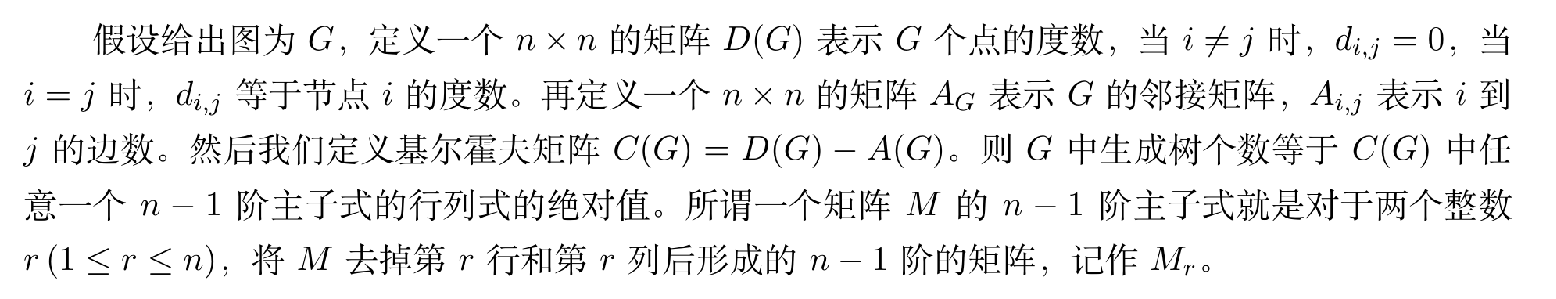
\includegraphics[width=8.92449822904368cm,height=1.715905030985808cm]{/home/xade/icpc/kactl/content/combinatorial/1.pdf}}
\raisebox{0.0\height}{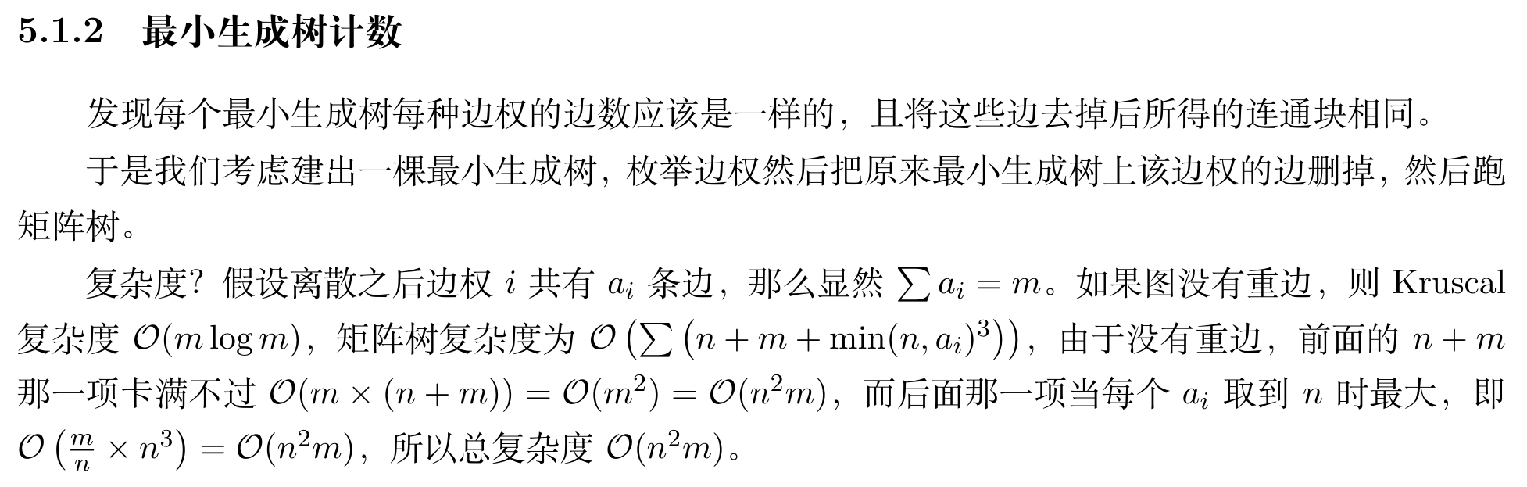
\includegraphics[width=8.92449822904368cm,height=2.845425996261112cm]{/home/xade/icpc/kactl/content/combinatorial/2.pdf}}



\subsubsection{Games.}
\begin{tmindent}
  Nim Game. Pick stone from k pile, at least 1, who cannot move lose. 
  XOR=0 lose.

  Bash Game. Pick stone from 1 pile, at least 1, at most m, who cannot move lose.
  n mod m+1=0 lose. apparent.

  Fib Game. Pick from k pile, at least 1, at most a[i]-1, at most previous taken*2, who cannot move lose.
  n is Fib lose. [?]

  Wythoff's Game. Pick from 2 piles, either pick 1 from any, or pick t from each pile (hence picking 2t elements, t is determined by player, t>1). cannot move lose.
  case discuss lead to $a[k] = (int)((b[k] - a[k]) * 1.618)$ where 1.618 is golden ratio
    
\end{tmindent}